\documentclass{boi2014-fi}

\usepackage{enumitem}

\renewcommand{\DayNum}{2}
\renewcommand{\TaskCode}{postmen}
\renewcommand{\TaskName}{Eläkeläisposteljoonit}

\begin{document}
    \begin{wrapfigure}[8]{r}{4cm}
        \vspace{-18pt}
        \includegraphics[width=4cm]{\TaskCode.jpeg}
    \end{wrapfigure}
    
    On vuosi 2036 ja Eurooppa on täpötäynnä eläkeläisiä. Pitääkseen
    heidät terveinä, Euroopan enemmistöministeri (eläkeläiset ovat
    enemmistö!) ehdottaa että eläkeläisten tulisi toimittaa se pieni määrä
    postia jota vielä lähetetään --- tyypillisesti eläkeläisille. Tämä ehdotus
    toteutetaan kaikkialla Euroopassa, jopa Norjan ja Sveitsin Vapaissa Valtioissa.
    
    Ministeriö on laatinut "eläkeläisposteljoonijärjestelmän" seuraavasti:
    Eurooppa on jaettu postialueisin. Postialueella on katuverkko joka muodostuu
    kaduista ja risteyksistä. Jokainen katu verkossa voidaan kävellä molempiin 
    suuntiin. Jokaisella alueella mielivaltainen määrä eläkeläisiä on saatavilla
    posteljooneiksi. Joka aamu jokainen posteljooni saa laukun, joka sisältää
    postia joka jaetaan kierrokselle joka peittää osan katuverkosta. Jokaisen
    kierroksen tulee olla eläkeläisyhteensopiva, eli sen on täytettävä seuraavat
    ehdot:
    \begin{itemize}
        \item Se alkaa ja loppuu samaan risteykseen. (Sehän on kierros!)
        \item Se ei kulje saman risteyksen läpi useammin kuin kerran. (Tällä
            tavalla eläkeläisposteljoonit eivät mene sekaisin reitistä.)
        \item Se ei saa kulkea samaa katua jonkin toisen kierroksen kanssa;
            tästä seuraa, että kaikkia katuja palvelee täsmälleen yksi
            posteljooni. (Tällä tavalla eläkeläisposteljoonit eivät tappele
            keskenään.)
    \end{itemize}

    Yhdesä kierrosten tulee peittää koko verkko: jokaisen verkon kadun tulee
    olla osa täsmälleen yhtä kierrosta.

    \Task
    Nyt ministeriö tarvitsee tietokoneohjelman, joka laskee postialueen katuverkon 
    kartasta joukon eläkeläisyhteensopivia kierroksia jotka peittävät verkon.

    \Input
    Syöte kuvaa katuverkon.
    
    Syötteen ensimmäinen rivi sisältää kaksi kokonaislukua $N$ ja $M$. $N$ on
    risteysten lukumäärä, ja $M$ on katujen lukumäärä. Risteykset numeroidaan
    luvuilla $1\ldots N$.

    Jokainen seuraavista $M$ rivistä sisältää kaksi kokonaislukua $u$ ja $v$
    ($1 \le u, v \le N, u \neq v$), jotka tarkoittavat että katu yhdistää
    risteyksiä $u$ ja $v$.

    Kaikille syötteille pätee:
    \begin{enumerate}
        \item Voit kulkea mistä tahansa risteyksestä mihin tahansa risteykseen.
        \item Ratkaisu on olemassa, eli voidaan löytää joukko eläkeläisyhteensopivia
            kierroksia jotka täyttävät verkon.
    \end{enumerate}
    
    \Output
    Tulosteen tulisi sisältää sama määrä rivejä kuin on eläkeläisyhteensopivia
    kierroksia.
    
    Tulosteen jokainen rivi sisältää kierroksen risteysten tunnusnumerot. Ne
    tulee antaa siinä järjestyksessä kuin missä posteljooni kulkee niiden
    läpi siten, että ensimmäinen (ja samalla viimeinen) risteys tulostetaan ensin
    (ja vain kerran).

    \Example

    \example
    {
        10 15 \newline
        1 3 \newline
        5 1\newline
        2 3 \newline
        9 2\newline
        3 4 \newline
        6 3\newline
        4 5 \newline
        7 4\newline
        4 8 \newline
        5 7 \newline
        8 5\newline
        6 7 \newline
        7 8 \newline
        8 10 \newline
        10 9
    }
    {
        2 3 4 5 8 10 9 \newline
        4 7 8 \newline
        1 5 7 6 3
    }
    {
        Seuraava kuvio kuvaa katuverkkoa ja kolmea eläkeläisyhteensopivaa
        kierrosta joilla se peitetään.

        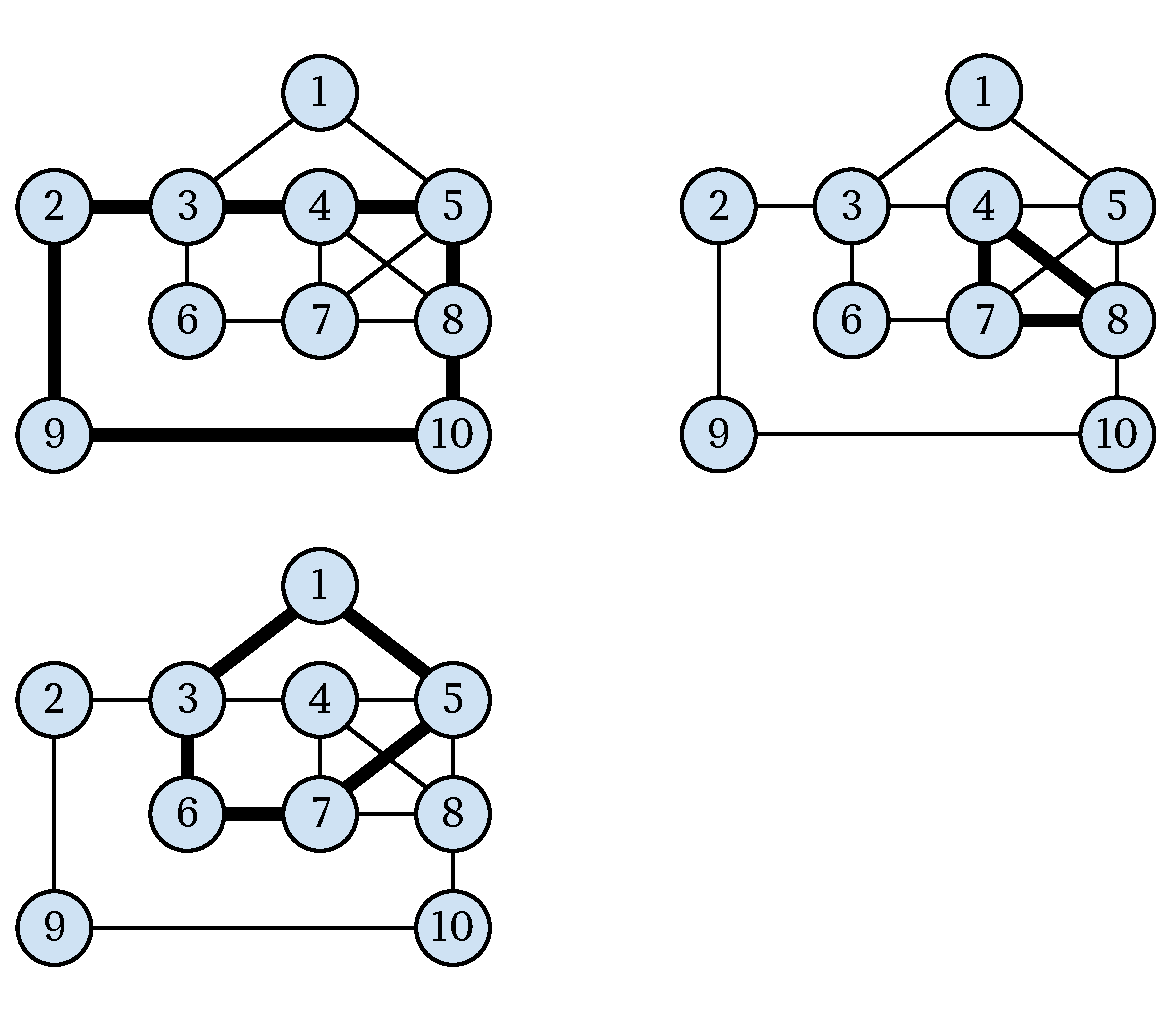
\includegraphics[width=7cm]{senior-example}

        Huomaa, että tähän esimerkkiin on useita ratkaisuja, niiden joukossa
        joitain sellaisia joissa on vain kaksi kierrosta.
    }

    \Scoring

    \begin{description}
        \item[Osatehtävä 1 (40 points):] $1 \le N \le 2\ 000$, $1 \le M \le 100\ 000$.
        \item[Osatehtävä 2 (20 points):] $1 \le N \le 100\ 000$, $1 \le M \le 100\ 000$.
        \item[Osatehtävä 3 (40 points):] $1 \le N \le 500\ 000$, $1 \le M \le 500\ 000$.
    \end{description}

    \Constraints

    \begin{description}
        \item[Aikaraja:] 1 s.
        \item[Muistiraja:] 256 MB.
    \end{description}

\end{document}
